%%%%%%%%%%%%%%%%%%%%%%%%%%%%%%%%%%%%%%%%%
% Ay 190 - WS2
% Written by Chatarin Wong-u-railertkun
%%%%%%%%%%%%%%%%%%%%%%%%%%%%%%%%%%%%%%%%%

%----------------------------------------------------------------------------------------
%	PACKAGES AND OTHER DOCUMENT CONFIGURATIONS
%----------------------------------------------------------------------------------------

\documentclass[11pt,letterpaper]{article}

% Load some basic packages that are useful to have
% and that should be part of any LaTeX installation.
%

\usepackage{graphicx}     % be able to include figures

\usepackage{xcolor}         % get nice colors

% change default font to Palatino (looks nicer!)
\usepackage[latin1]{inputenc}
\usepackage{mathpazo}
\usepackage[T1]{fontenc}

% load some useful math symbols/fonts
\usepackage{latexsym,amsfonts,amsmath,amssymb}
\usepackage{subcaption}

% comfort package to easily set margins
\usepackage[top=1in, bottom=1in, left=1in, right=1in]{geometry}

% control some spacings
%
% spacing after a paragraph
\setlength{\parskip}{.15cm}
% indentation at the top of a new paragraph
\setlength{\parindent}{0.0cm}

\usepackage{courier}


%----------------------------------------------------------------------------------------
%	TITLE
%----------------------------------------------------------------------------------------

\begin{document}

\begin{center}
\Large
Ay190 -- Worksheet 07: Monte Carlo \\    %%%%%% DON'T FORGET TO CHANGE THE WORK SHEET NUMBER
Chatarin (Mee) Wong-u-railertkun\\
Date: \today
\end{center}

\section{Estimation of Pi}

\begin{figure}[h!]
	\centering
	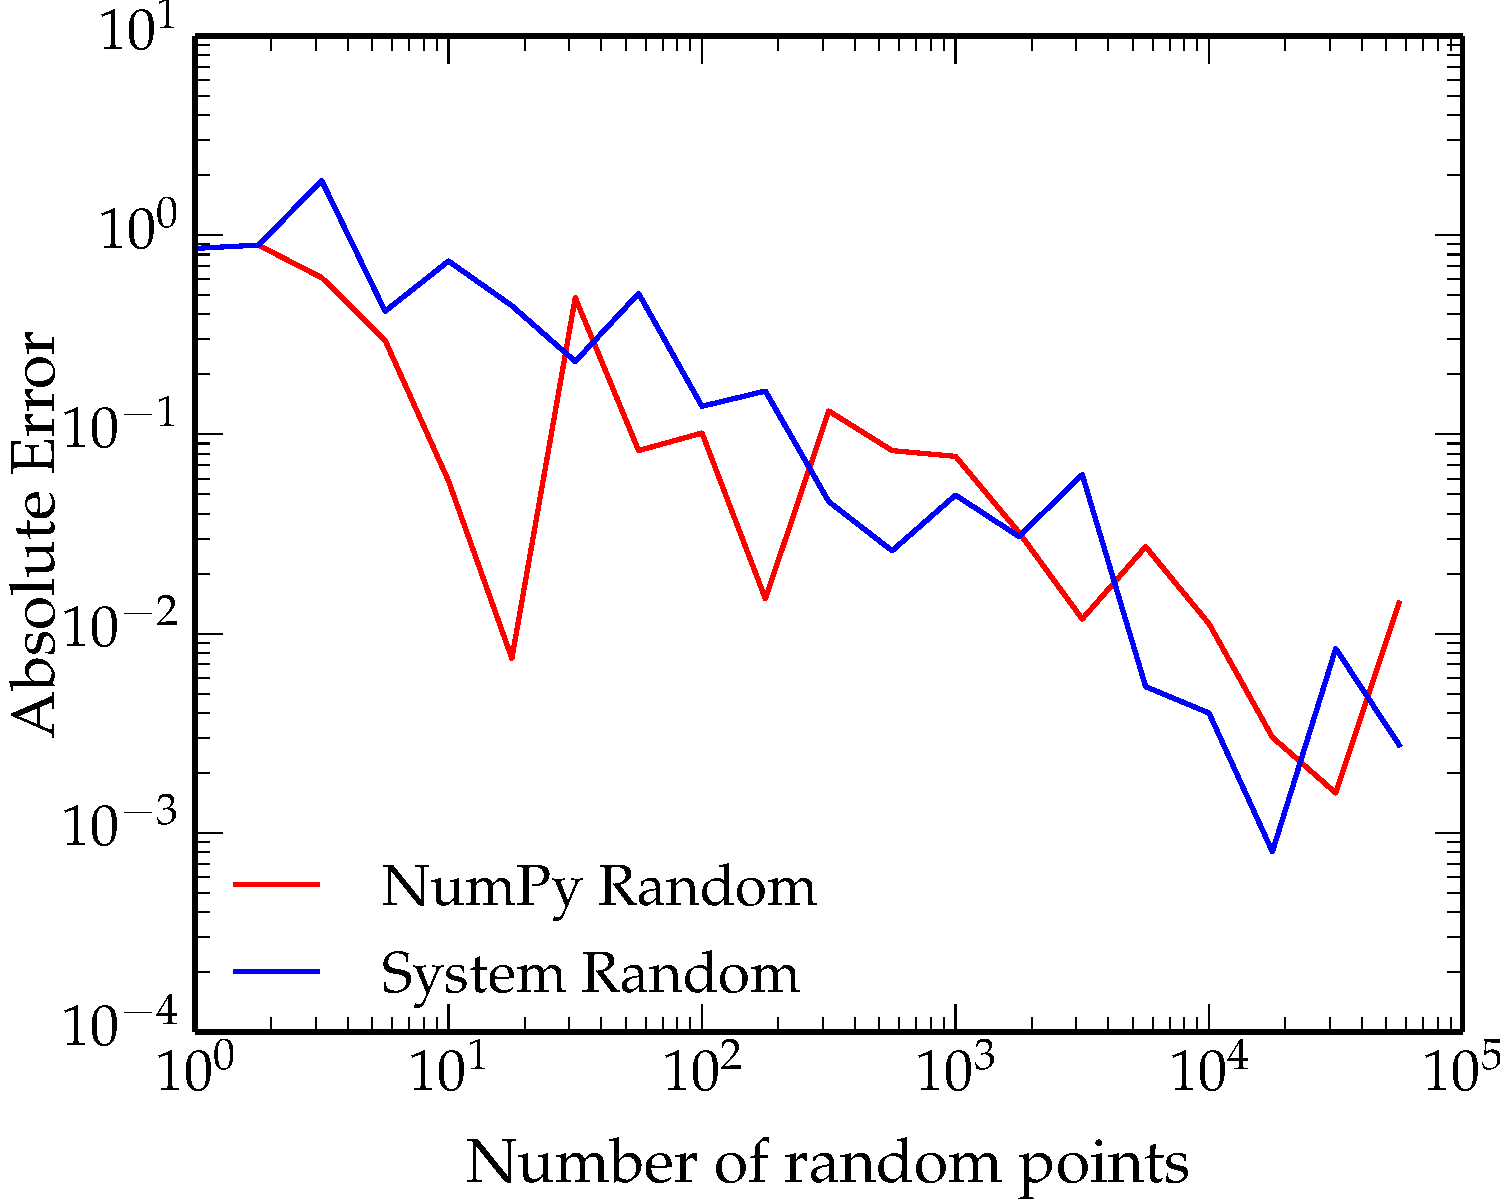
\includegraphics[width=0.5\textwidth]{EstPi}
	\caption{Absolute error of estimation of pi, using monte carlo method, with two types of random generator, \texttt{Numpy} and \texttt{System} random.}
	\label{fig:EstPi}
\end{figure}
	
Using Monte Carlo to calculate the value of pi, based on the steps in the lecture note. We can see that the lines are not smooth, because we are dealing with
random numbers. However, we can see that the errors have the trend of decreasing, as number of points increases. In this circumstances, there is not much difference between using \texttt{Numpy} or \texttt{System} random generator, may be because the number of points is not big enough that the \texttt{Numpy} random completes the cycle.

\section{Birthday Paradox}

\begin{figure}[h!]
	\centering
	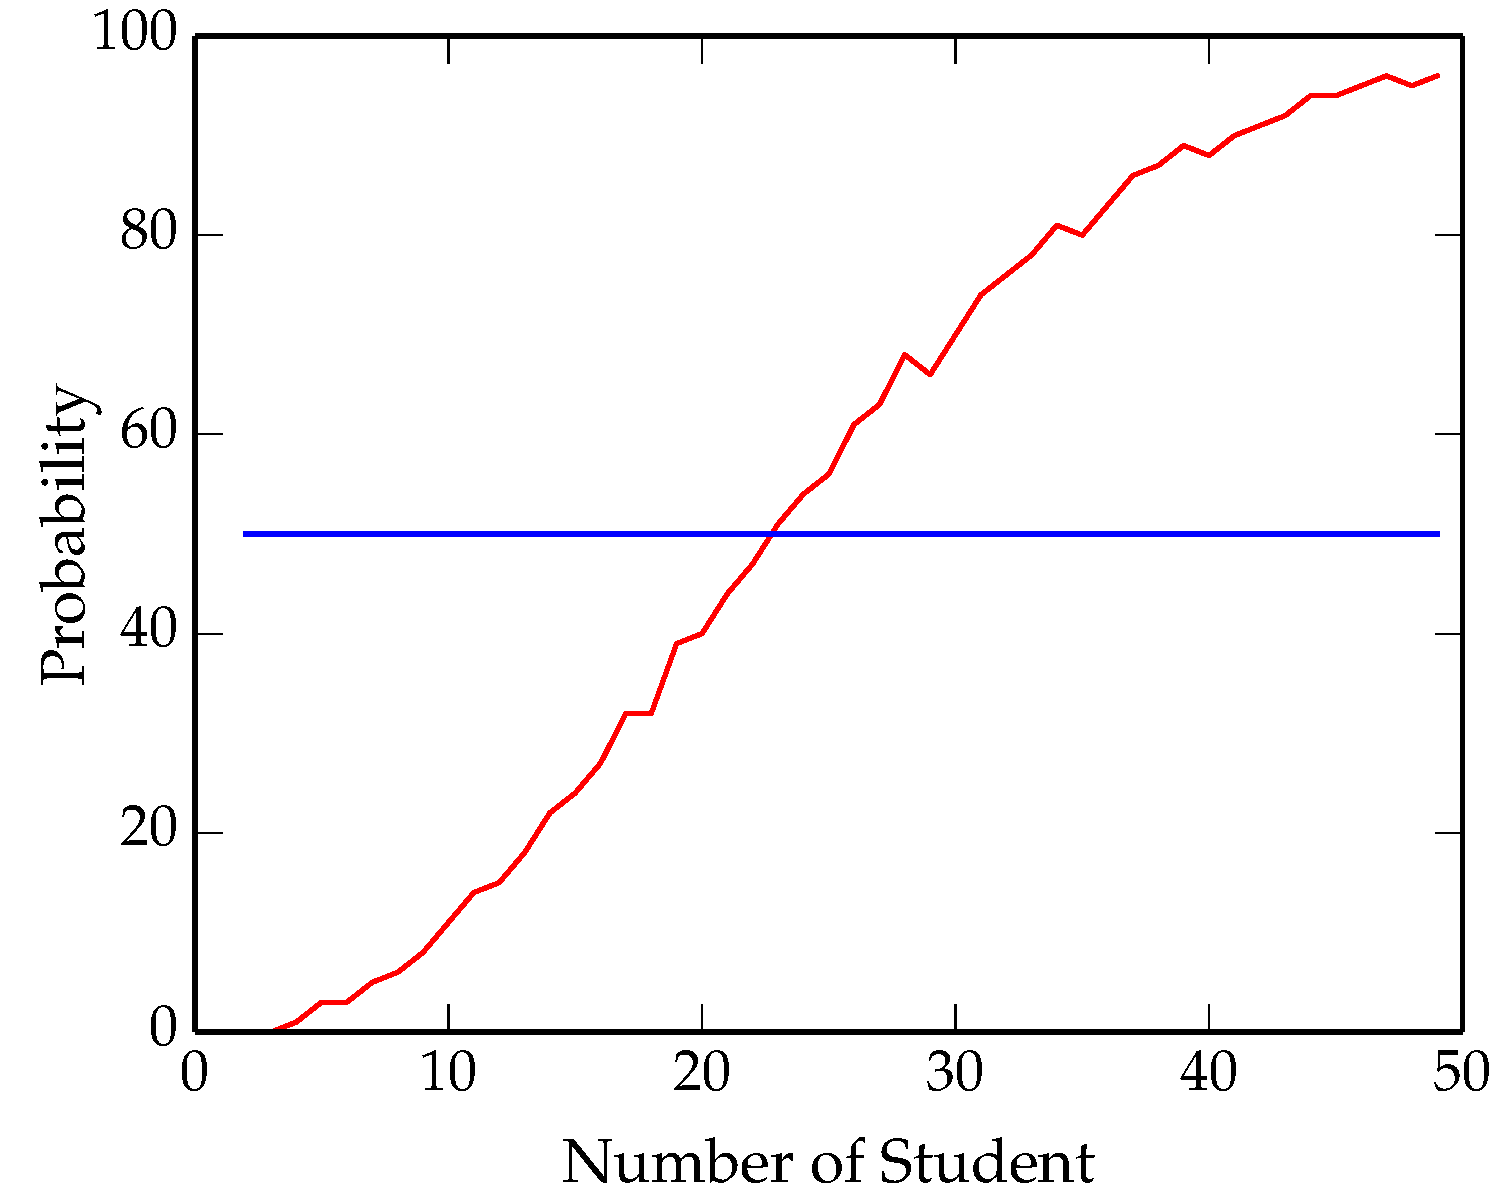
\includegraphics[width=0.5\textwidth]{Birthday}
	\caption{Probability of having at least 2 people with the same birthday vs. the group size. The probability goes over 50\% at 23 people.}
	\label{fig:Birthday}
\end{figure}

In figure \ref{fig:Birthday}, we can see that when number of people reaches 23, the probability of having at least 2 people with the same birthday increases over 50\%. That number matches with the answer given from the internet search, which derived from the law of probability, instead of Monte Carlo. It's amazing to see that, even at low number of people as 50, it's almost guarantee that at least 2 people will have the same birthday.

\newpage
\section{More MC Integration}

\begin{figure}[h!]
	\centering
	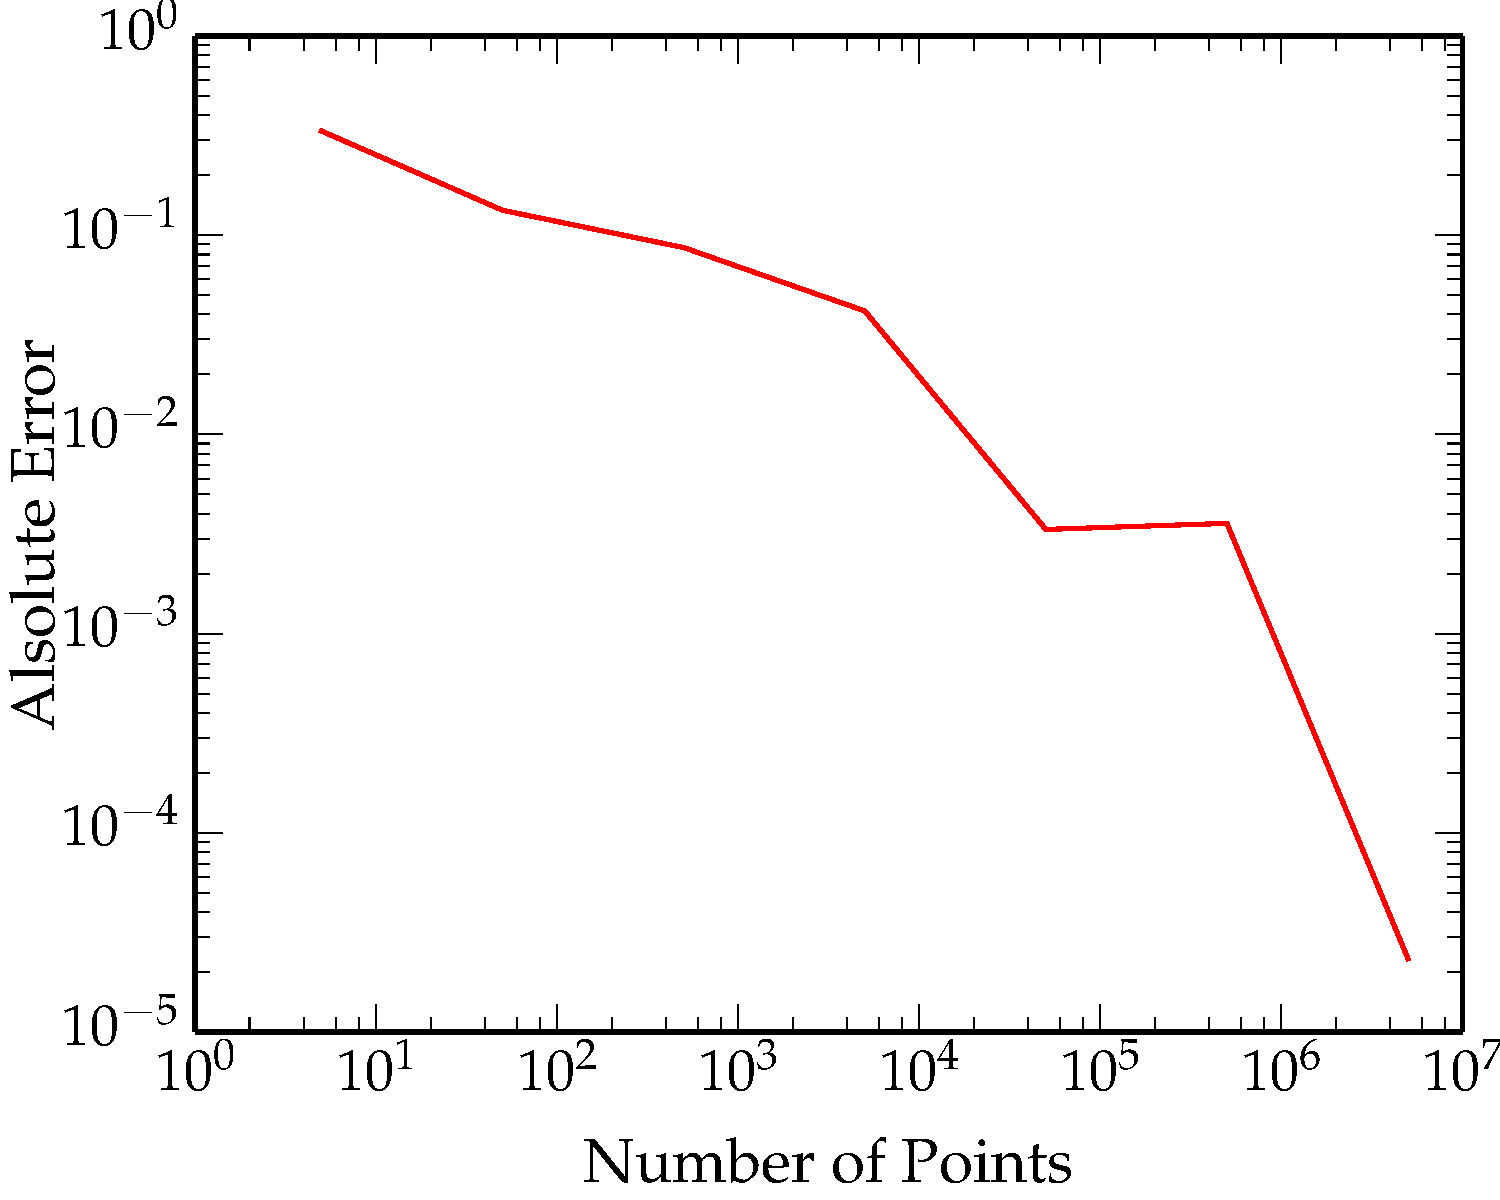
\includegraphics[width=0.5\textwidth]{HitMiss}
	\caption{Error of the integral using the hit-or-miss Monte Carlo.}
	\label{fig:HitMiss}
\end{figure}

The exact answer of the integral in question is 22/3. We can see that the error is close to $\propto N^{-0.5}$, as expected.

\end{document}

